\documentclass[11pt,letterpaper]{article}
\usepackage[utf8]{inputenc}
\usepackage[spanish,USenglish]{babel}
\usepackage{amsmath}
\usepackage{amsfonts}
\usepackage{amssymb}
\usepackage{amsthm}
\usepackage{graphicx}
\usepackage[left=2cm,right=2cm,top=2cm,bottom=2cm]{geometry}
\usepackage{flushend}
\usepackage{pgf,tikz, pgfplots}
\usetikzlibrary{arrows}
\pgfplotsset{compat=1.15}
\usepackage{pgf,tikz,pgfplots}
%escribir programas
\usepackage{listings}
\usepackage{algpseudocode}
\usepackage{algorithm}
\renewcommand{\algorithmicrequire}{\textbf{Input:}}
\renewcommand{\algorithmicensure}{\textbf{Output:}}

%encabezado
\usepackage{fancyhdr}
\pagestyle{fancy}
\fancyhf{}
\fancyhead[RO]{\thepage} % Números de página en las esquinas de los encabezados
%%%%%%%%%%%%%%%%%%%% BOXES %%%%%%%%%%%%%%%%%%%
\usepackage{bm}
\newcommand{\commentedbox}[2]{%
	\mbox{
		\begin{tabular}[t]{@{}c@{}}
			$\boxed{\displaystyle#1}$\\
			#2
		\end{tabular}%
	}%
}
\usepackage{framed}
\usepackage{wrapfig}\definecolor{shadecolor}{RGB}{224,238,238}
%%%%%%%%%%%%%%%%%%%%%%%%% DEFINITIONS %%%%%%%%%%%%%%%%%%%%%%%%
\theoremstyle{definition}
\newtheorem{defi}{Definición}[section]%Para definiciones
\theoremstyle{definition}
\newtheorem{teo}{Teorema}[section]%Para definiciones
\newtheorem{prop}{Proposición}
\theoremstyle{definition}
\newtheorem{ej}{Ejemplo}[section]
\newtheorem{lem}{Lema}
\newtheorem{prblm}{Problema}
\newtheorem{col}{Corolario}[section]



\title{\textbf{Tarea 5: Descenso Gradiente Parte 2}\\ Optimización I \\ \Large {Maestría en Computación}\\ \Large {Centro de Investigación en Matemáticas}}
\author{Esteban Reyes Saldaña \\ esteban.reyes@citmat.mx}

\begin{document}

\selectlanguage{spanish}
\twocolumn[
\begin{@twocolumnfalse}
	\maketitle
	\begin{center}\rule{0.9\textwidth}{0.1mm} \end{center}
	\begin{abstract}
		\normalsize{En esta tarea se utilizó el método de descneso gradiente para maximixar la función log-likelihood del dataset \textit{mnist.pkl.gz}. La función log-likelihood es conocida en la literatura por su capacidad de clasificación binaria. En este caso el conjunto de datos corresponde a imágenes de números dígitos escritos a mano. Para maximizar esta función se minimizó su negativo. Se presenta a continuación una descripción general la función log-likelihood, así como el pseudocódigo de los métodos implementados. En los resultados se incluyen pruebas de descenso gradiente tanto como para búsqueda por backtracking y bisección.Finalmente se incluyen conclusiones observadas a partir de la experimentación.}
	\begin{center}\rule{0.9\textwidth}{0.1mm} \end{center}
	\end{abstract}
\end{@twocolumnfalse}]

\section{Introducción}
\subsection{Función Log-Likelihood}
Dado un conjunto de datos de entrenamiento, 
\[\{x_i, y_i\}_{i = 1}^n\]
donde $ y_i \in \{ 0,1 \} $, la función \textbf{log-likelihood} está dada por
\begin{shaded*}
\begin{eqnarray*}
	H ( \beta, \beta_0) & = & \sum_{i = 1}^n y_i \log(\pi_i) + ( 1 - y_i) \log(1-\pi_i) \\
	\pi_i (\beta, \beta_0) & = & \dfrac{1}{1 + \exp (-x_i^T \beta - \beta_0)}
\end{eqnarray*}
\end{shaded*}
Sea $ m = dim(x_0) = dim(x_1) = \dots, dim(x_n) $. Notemos que $ \beta \in\mathbb{R}^m $ y $ \beta_0 \in \mathbb{R} $. Entonces, por motivos prácticos y como más adelante estaremos interesados en calcular el gradiente con respecto a los valores beta se introduce el cambio de variable,
\begin{equation}
	\phi = [\beta, \beta_0]^T
\end{equation}
como el vector que concatena a $ \beta $ y a $ \beta_0 $. Además
\begin{eqnarray*}
	- x_i^T \beta - \beta_0 & = &- \left[x_i^1, x_i^2, \dots, x_i^m \right] 
								\left[\begin{matrix}
									\beta_1 \\
									\vdots \\
									\beta_m
								\end{matrix}\right] - \beta_0 \\
							& = & - \left[x_i^1, x_i^2, \dots, x_i^m, 1 \right] 
								\left[\begin{matrix}
									\beta_1 \\
									\vdots \\
									\beta_m \\
									\beta_0
								\end{matrix}\right] \\
							& = & - \hat{x}_i^T \phi.
\end{eqnarray*}
Entonces reescribimos $ h(\beta, \beta_0) $ como 
\begin{shaded*}
	\begin{eqnarray*}
		H ( \phi) & = & \sum_{i = 1}^n y_i \log(\pi_i) + ( 1 - y_i) \log(1-\pi_i) \\
		\pi_i (\phi) & = & \dfrac{1}{1 + \exp (-\hat{x}_i^T \phi)}
	\end{eqnarray*}
\end{shaded*}
Algunos resultados relevantes sobre el gradiente, vistos en la tarea pasada son
\begin{shaded*}
\begin{teo}
	Sea $ f: \mathbb{R}^n \to \mathbb{R} $ una función continuamente diferenciable. Entonces para toda $ x  \in dom(f) $, $ \nabla f(x) $ es perpendicular al conjunto de nivel
	\[ S = \{ x \in \mathbb{R}^n | f(x) = c, c\textup{ constante.} \} \]
\end{teo}
\end{shaded*}

\begin{shaded*}
\begin{teo}\label{max_}
	Sea $ f: \mathbb{R}^n \to \mathbb{R} $ una función continuamente diferenciable. Entonces la dirección donde $ f(x) $ crece más rápido es $ \nabla f(x) $.
\end{teo}
\end{shaded*}

\begin{col}
	Bajo las condiciones del Teorema (\ref{max_}), $ f(x) $ decrece más rápido en la dirección $ - \nabla f(x) $.
\end{col}

\begin{shaded*}
\begin{defi}
	Una \textbf{dirección de descenso} $ d \in \mathbb{R}^n $ para $ f \in \mathcal{C}^1 $ es un vector tal que
	\[ f(x + t d) < f(x) \]
	para $ t \in (0, T) $. Es decir, permite que el punto $ x $ más cerca al mínimo local $ x^* $ de la función objetivo $ f: \mathbb{R}^n \to \mathbb{R} $.
\end{defi}
\end{shaded*}

\begin{shaded*}
\begin{teo}
	Si $ g(x)^T d < 0 $ entonces $ d $ es una dirección de descenso.
\end{teo}
\end{shaded*}
\textbf{Observación.} La dirección 
\[ d_k = - g(x_k) \]
es la elección más obvia de una dirección de búsqueda.
\\
\textbf{Observación.} El objetivo es \textbf{maximizar} la función $ h(\phi) $ usando descenso gradiente. Por los resultados anteriores es fácil ver que esto es equivalente a \textbf{minimizar} $ -h(\phi) $.
\section{Datos MNIST}
Los datos utilizados corresponden a la base de datos MNIST. Que son imágenes de números dígitos escritos a mano. Las imágenes tiene  dimensión $ 28 \times 28 $ y la distribución de los datos está dada por
\begin{center}
	\begin{tabular}{|c|c|}
	\hline
	Datos & Cantidad \\
	\hline
	Entrenamiento & 50000 \\
	\hline
	Pruebas & 10000 \\
	\hline
	Validación & 10000 \\
	\hline
\end{tabular}
\end{center}
A continuación se muestra un ejemplo del conjunto de entrenamiento
\begin{center}
	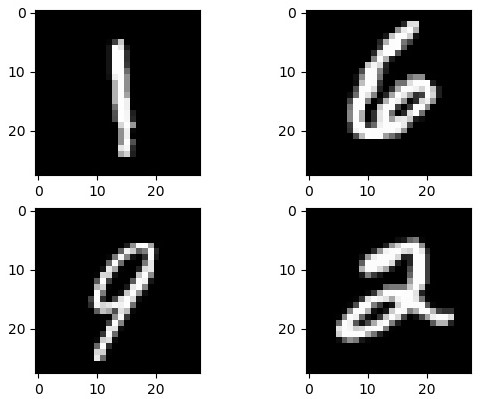
\includegraphics[width=0.8\linewidth]{graficas/example}
\end{center}
Dado que la función $ h(\phi) $ corresponde a clasificación binaria, la experimentaición se realizó con las imágenes de etiqueta cero y uno.
\section{Método}
\subsection{Gradiente}
Usando la relación derivada-gradiente y regla de la cadena tenemos que
\begin{eqnarray*}
	\nabla \pi_i (\phi) & = & - \dfrac{\exp(-\hat{x}_i^T \phi)}{[1 + \exp(-\hat{x}_i^T \phi)]^2} \hat{x}_i \\
						& = & - \dfrac{1 + \exp(-\hat{x}_i^T \phi) - 1}{[1 + \exp(-\hat{x}_i^T \phi)]^2} \hat{x}_i
\end{eqnarray*}

\begin{eqnarray*}
	& = & \left(- \dfrac{1}{1 + \exp(-\hat{x}_i^T \phi)}  + \dfrac{1}{[1 + \exp(-\hat{x}_i^T \phi)]^2}\right) \hat{x}_i \\
	& = & [- \pi_i(\phi) + \pi_i^2 (\phi)] \hat{x}_i \\
	& = & (1 -  \pi_i(\phi))  \pi_i(\phi) \hat{x}_i.
\end{eqnarray*}
Así que
\begin{shaded*}
	\begin{equation}
		\nabla \pi_i (\phi) = (1 -  \pi_i(\phi))  \pi_i(\phi) \hat{x}_i.
	\end{equation}
\end{shaded*}
Ahora,
\begin{eqnarray*}
	\nabla h(\phi) & = & \sum_{i = 1}^n \left[ y_i \dfrac{\nabla \pi_i(\phi)}{\pi_i(\phi)} + ( 1 - y_i)\dfrac{\nabla (1 - \pi_i(\phi))}{1 - \pi_i(\phi)}  \right] \\
				   & = & \sum_{i = 1}^n \left[ y_i \dfrac{(1 - \pi_i(\phi)) \pi_i(\phi) \hat{x}_i}{\pi_i(\phi)} \right. \\
				   &   & \left. - ( 1 - y_i)\dfrac{(1 - \pi_i(\phi)) \pi_i(\phi) \hat{x}_i}{1 - \pi_i(\phi)}  \right] \\
				   & = & \sum_{i = 1}^n \left[ y_i (1 - \pi_i(\phi)) \hat{x}_i  - ( 1 - y_i) \pi_i(\phi) \hat{x}_i  \right] 
\end{eqnarray*}
Entonces
\begin{shaded*}
\begin{equation*}
	\nabla h(\phi) = \sum_{i = 1}^n \left[ y_i (1 - \pi_i(\phi)) \hat{x}_i  - ( 1 - y_i) \pi_i(\phi) \hat{x}_i  \right] 
\end{equation*}	
\end{shaded*}
\subsection{Pseudocódigo}
\subsubsection{Búsqueda con BackTracking}
\begin{shaded*}
	\begin{algorithmic}[1]
		% ENTRADA / SALIDA
		\Require{$ \hat{\alpha} $, $ \rho \in (0,1) $, $ c_1 \in (0,1) $}
		\Ensure{Tamaño de paso $ \alpha_k $}
		\State{Haga $ alpha = \hat{\alpha} $}
		\State{$inum =0 $}
		\While{$ f(x_k + \alpha d_k) > f(x_k) + c_1 \alpha \nabla f_k^T d_k $}
			\State{$ alpha \to \rho \alpha $}
		\EndWhile
		\State{Regresa $ \alpha_k = \alpha $}
	\end{algorithmic}
\end{shaded*}

\subsubsection{Búsqueda en Línea con Bisección}
\begin{shaded*}
	\begin{algorithmic}[1]
		% ENTRADA / SALIDA
		\Require{$ \alpha_0 $, $ 0 < c_1 < c_2 < 1 $}
		\Ensure{Tamaño de paso $ \alpha_k $}
		\State{Haga $ alpha = 0 $, $ \beta = \infty $, $ \alpha^i = \alpha_0 $}
		\State{$inum =0 $}
		\While{$ f(x_k + \alpha_k d_k) > f(x_k) + c_1 \alpha_k \nabla f_k^T d_k $ \textbf{o} $ \nabla f(x_k + \alpha_k d_k)^T d_k < c_2 \nabla f(x_k)^T d_k $}
			\If{$ f(x_k + \alpha_k d_k) > f(x_k) + c_1 \alpha_k \nabla f_k^T d_k $}
				\State{$ \beta = \alpha_k $}
				\State{$ \alpha_k = \dfrac{\alpha + \beta}{2} $}
			\Else
				\State{$\alpha = \alpha_k $}
				\If{$\beta = \infty $}
					\State{$\alpha_k = 2 \alpha$}
				\Else
					\State{$ \alpha_k = \dfrac{\alpha + \beta}{2} $}
				\EndIf
			\EndIf
		\EndWhile
		\State{Regresa $ \alpha_k $}
	\end{algorithmic}
\end{shaded*}


\section{Resultados}
Del conjunto de entrenamiento se usaron un total de $ 10,610 $ ejemplos de dígitos cero y uno. Como vector inicial se usó $ \beta = [1, \dots, 1]^T $, $ \beta_0 = 1 $ y para los algoritmos de búsqueda en línea se usaron los parámetros
\begin{center}
	\begin{tabular}{cc}
		\hline
		Parámetro & Valor \\
		\hline
		$\alpha $ & 0.9 \\
		$ \rho $  & 0.5 \\
		$ c_1 $ & $ 10^{-4} $ \\
		$ c_2 $  & $ 0.9 $ \\
		\hline
	\end{tabular}
\end{center}
Para un máximo de $ 500 $ iteraciones se obtuvo
\begin{center}
	\begin{tabular}{ccc}
		\hline
		Algoritmo & $ || G_k || $ & tiempo \\
		\hline
		BackTracking & 0.0166 & 228.86 segundos \\
		Bisección    & 0.0053 & 494.09 segundos \\
		\hline
	\end{tabular}
\end{center}
\newpage
Para medir el error se usó la función
\begin{shaded*}
$$ error = \dfrac{1}{n} \sum_{i=1}^n | \textbf{1} _{\pi(\hat{\beta}, \hat{\beta}_0) > 0.5 }(x_i) - y_i | $$
donde $ \{ (x_i, y_i) \}_{i = 1} ^n  $ se obtiene del conjunto train\_set y $ x_i \in \mathbb{R}^{784} $ y $ y_i \in \{ 0, 1\} $.
\end{shaded*}
Para el punto mínimo encontrado en la experimentación se obtuvo
\begin{center}
	\begin{tabular}{cc}
		\hline
		Algoritmo    & $ error $  \\
		\hline
		BackTracking & 0.0047  \\
		Bisección    & 0.0047  \\
		\hline
	\end{tabular}
\end{center}
\begin{center}
Gráficas para Backtracking
\\
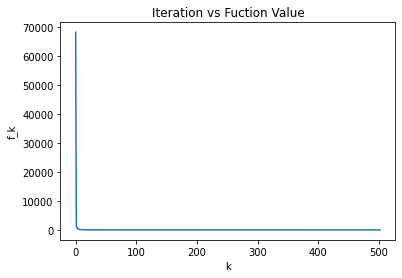
\includegraphics[width=0.8\linewidth]{graficas/bt_f}
\\
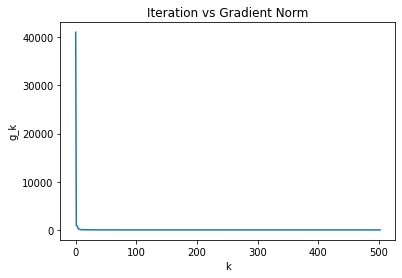
\includegraphics[width=0.8\linewidth]{graficas/bt_g}
\\
Gráficas para Bisección
\\
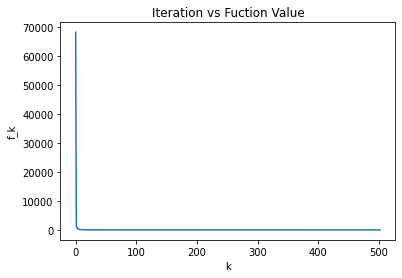
\includegraphics[width=0.8\linewidth]{graficas/bic_f}
\\
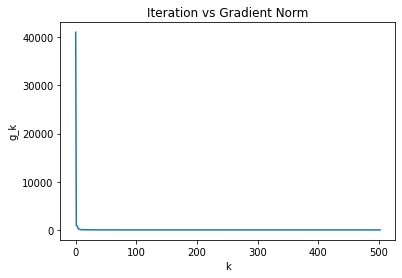
\includegraphics[width=0.8\linewidth]{graficas/bic_g}
\end{center}

\section{Conclusiones}
	\begin{itemize}
		\item El problema de clasificación binaria de un conjunto de entrenamiento se puede plantear como un problema de optimización. En este caso se usó la función de log-likelihood para clasificar un conjunto de imágenes de ceros y unos del dataset MNIST. 
		\item En la experimentación se observó que el método de backtracking convergió en menor tiempo comparado con el método de bisección. La norma del gradiente quedó más cerca de cero para bisección y el error obtenido para ambos métodos se mantuvo igual.
		\item Observemos que el error es pequeño, considerando el número total de imágenes del conjunto de validación. Intuitivamente esto puede ocurrir porque la clasificación es clara para ceros y unos (dado que la forma de escribir estos dígitos es muy diferente). Lo que sugiere probar este algoritmo para clasificar unos y sietes o seis y nueves.
	\end{itemize}
\end{document}